
\section{Methodology and Results}
We used the simulation framework~\cite{spock13} used previously for TTR studies~\cite{carterkorbel13} to generate TTR results. 
In addition, we implemented a web-based visualization tool that was used to generate all of the figures in this paper.
For each figure, note that the legend identifies each simulation as follows:
\begin{verbatim}
benchmark.policy.setbits-linebits-associativity
\end{verbatim}
where \texttt{benchmark} is the application trace being used, 
\texttt{policy} describes how the cache chooses how to replace lines when there is a conflict, 
and \texttt{setbits}, \texttt{linebits}, and \texttt{associativity} all represent the cache configuration for a particular simulation.

The procedure for interpreting TTR curves is as follows. First, we choose to hold the cache size constant. With this constraint, we have three parameters that can be varied, the number of sets, the line length, and the number of ways (associativity). As discussed above, a cache configuration is shown as (set bits)\_(line bits)\_(associativity ways). 
For example the configuration \texttt{5\_6\_4} has $2^5$ sets, $2^6$ bytes per line and 4 associativity ways. 
Because the cache size is held constant, an increase in any one parameter must be accompanied by a decrease in another parameter. 
Thus, if we limit ourselves to varying as little as possible at a time, we have six possible ways to modify a cache configuration:

\begin{enumerate}
\item Increase associativity, decrease sets
\item Increase associativity, decrease line length
\item Increase sets, decrease line length
\item Increase sets, decrease associativity
\item Increase line length, decrease sets
\item Increase line length, decrease associativity
\end{enumerate}

From this, it is clear that without any insight into the direction that will lead to improvement, enumerating all possibilities would take exponential time! No need to fear, because TTR will allow us to apply heuristics to quickly converge on the optimal cache configuration. To demonstrate this in action, here's an example:

%sp_omp-srrip-6_6_8
\begin{figure}[ht]
\begin{center}
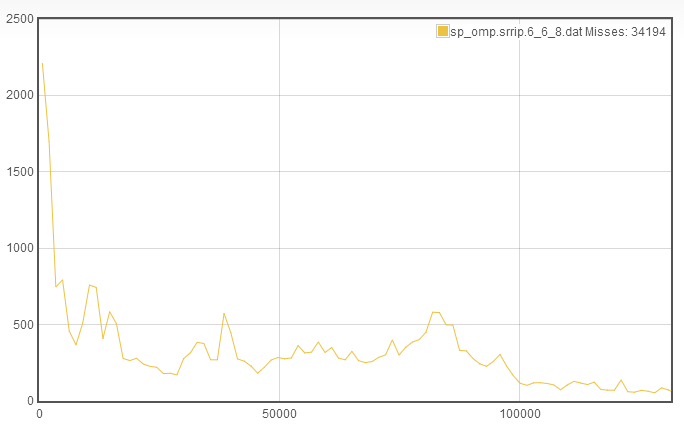
\includegraphics[width={0.9\columnwidth}]{images/sp_omp-srrip-6_6_8}
\end{center}
\caption{\texttt{sp\_omp.srrip.6\_6\_8}}
\label{6_6_8}
\end{figure}

For this case, we use \texttt{sp\_omp} from the NAS Parallel Benchmarks~\cite{bailey94}. Among the traces that we have access to, it is a relatively cache intensive program, which makes it a good candidate to optimize. Additionally, we only consider a single cache replacement policy at a time. So for this example, we search for the optimal cache configuration using the Static Re-reference Interval Prediction (SRRIP) replacement scheme from Jaleel et. al.~\cite{jaleeltheobald10}. To begin, we arbitrarily select the 
\texttt{6\_6\_8 } cache configuration. The TTR curve for this is in Figure~\ref{6_6_8}.

We begin by explaining the plot in Figure~\ref{6_6_8} for the uninitiated, since none of the plots in this paper have any axis labels, but they all use the same axes. The x axis is memory accesses to recache. Essentially, if a line is evicted from the cache and brought back in after a small number of memory access, it will end up close to the y axis. The y axis is the number of recache occurences of a particular duration that occur in the course of sampling. Note that the data is also bucketed and was sampled with a warmup period to remove cumpolsory misses. Notice in the legend that the series name is listed and includes the total misses, which we can use as a proxy for miss rate since the same number of cycles was run for each TTR curve we are comparing.

So, how do you interpret this graph? One thing to notice is what we call the rapid recaching (RR), which might also be referred to as thrashing. In this case, we see that among the roughly 34000 misses, only about 2200 were due to rapid recaching. This means that we can afford to decrease associativity and increase either the number of sets or the line length. Without any additional information, we have no good way to determine whether line length or set number should be increased. we found that by choosing either, it will eventually converge on the same answer. So for the purposes of brevity, we first increase the number of sets. This makes the new cache configuration \texttt{7\_6\_4} which is added in Figure~\ref{7_6_4}.

%7_6_4
\begin{figure}[ht]
\begin{center}
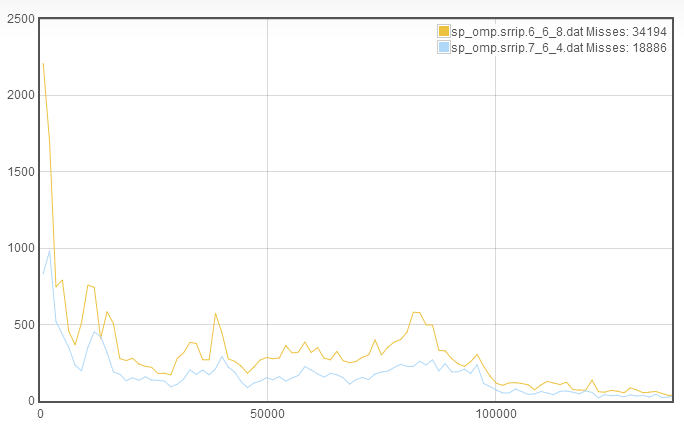
\includegraphics[width={0.9\columnwidth}]{images/sp_omp-srrip-7_6_4}
\end{center}
\caption{\texttt{sp\_omp.srrip.7\_6\_4}}
\label{7_6_4}
\end{figure}

From this, we see that there is a signficant decrease in misses and the decrease comes roughly equally from all parts of the TTR curve. Additionally, despite decreasing associativity, the rapid recaching is still quite low. This suggests that decreasing the associativity to increase the number of sets, this results in a cache configuration of \texttt{8\_6\_2}, which is added in Figure~\ref{8_6_2}.

%8_6_2
\begin{figure}[ht]
\begin{center}
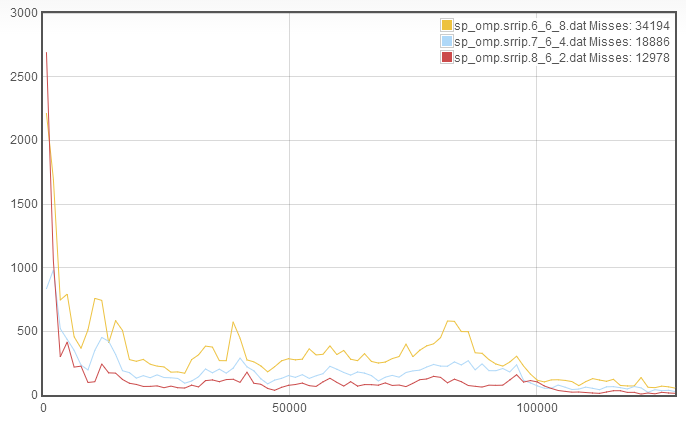
\includegraphics[width={0.9\columnwidth}]{images/sp_omp-srrip-8_6_2}
\end{center}
\caption{\texttt{sp\_omp.srrip.8\_6\_2}}
\label{8_6_2}
\end{figure}

We see that again we see an improvement in the misses. However, now the rapid recaching has skyrocketed! This suggests that the increase in number of sets was beneficial, but the decrease in associativity was detrimental. Therefore, we try to increase associativity at the expense of line length, which gives the new cache configuration \texttt{8\_5\_4} found in Figure~\ref{8_5_4}.

%8_5_4
\begin{figure}[h]
\begin{center}
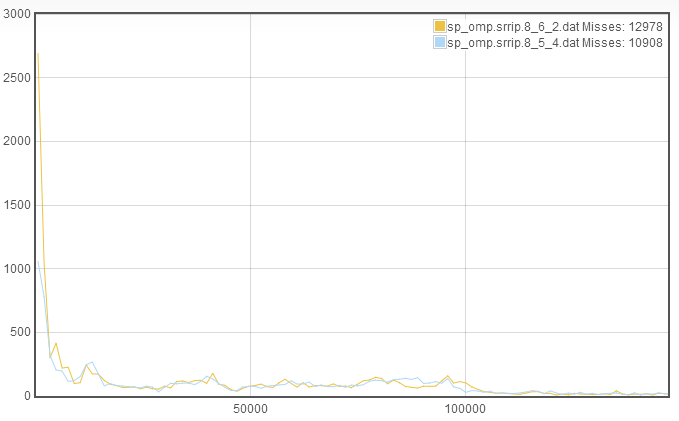
\includegraphics[width={0.9\columnwidth}]{images/sp_omp-srrip-8_5_4}
\end{center}
\caption{\texttt{sp\_omp.srrip.8\_5\_4}}
\label{8_5_4}
\end{figure}

We again see improvement in the number of misses, however in this case, the improvement is due almost entirely to a decrease in the rapid recaching. This suggests that we may have room to further decrease the line length. Since the rapid recaching is not significantly larger than the slower recaching, this suggests that we use the decreased line length to increase the number of sets, to get a new cache configuration of \texttt{9\_4\_4} in Figure~\ref{9_4_4}.

%9_4_4
\begin{figure}[h]
\begin{center}
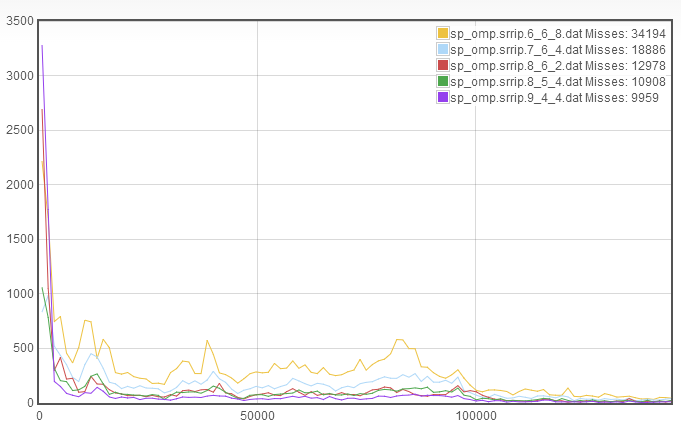
\includegraphics[width={0.9\columnwidth}]{images/sp_omp-srrip-9_4_4}
\end{center}
\caption{\texttt{sp\_omp.srrip.9\_4\_4}}
\label{9_4_4}
\end{figure}

We see very minor improvement in the misses, because the slower recache rates have gone down but the rapid recaching has skyrocketed. This suggests that we increase the associativity. Lacking any intuition for whether line length or number of sets should be decreased, we abritrarily choose to decrease the line length so that we now have \texttt{9\_3\_8} as in Figure~\ref{9_3_8}.

%9_3_8
\begin{figure}[h]
\begin{center}
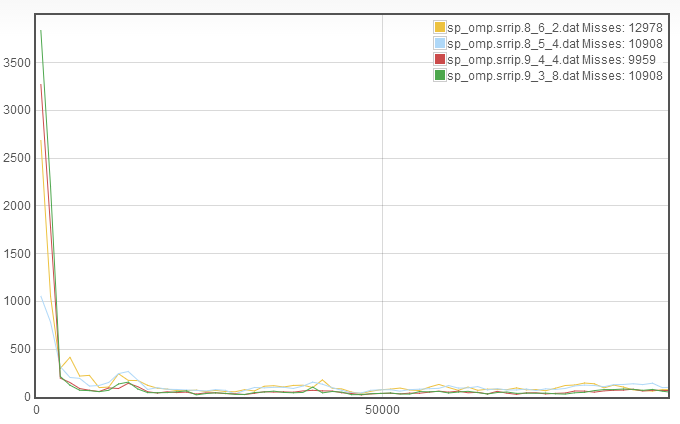
\includegraphics[width={0.9\columnwidth}]{images/sp_omp-srrip-9_3_8}
\end{center}
\caption{\texttt{sp\_omp.srrip.9\_3\_8}}
\label{9_3_8}
\end{figure}

We see that the miss rate increased. This is due to an increase in the rapid recaching without significant improvement in the slower recaches. This leaves the only reasonable place for improvement to be to go back to the \texttt{9\_4\_4} configuration and decrease the number of sets instead of the line length, to get \texttt{8\_4\_8} found in Figure~\ref{8_4_8}.

%8_4_8
\begin{figure}[h]
\begin{center}
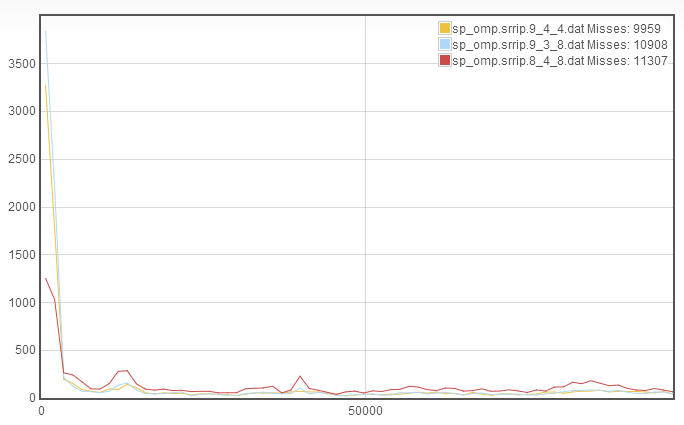
\includegraphics[width={0.9\columnwidth}]{images/sp_omp-srrip-8_4_8}
\end{center}
\caption{\texttt{sp\_omp.srrip.8\_4\_8}}
\label{8_4_8}
\end{figure}

We see that again there is not an improvement in misses relative to \texttt{9\_4\_4}. 
We find that the rapid recache went down considerably, however there is no way to increase the associativity that we have not already tested! So we conclude that the optimal cache configuration is \texttt{9\_4\_4}. Having run nearly all of the reasonable cache configurations, this does in fact appear to be the optimal cache configuration.

